\section{Introduction}

Today, it is difficult to produce high quality tools that support debugging
of OpenMP programs without tightly integrating them with a specific
OpenMP runtime implementation.
To address this problem, this document defines OMPD, an application
programming interface (API) for a shared-library plugin that will
enable debuggers to inspect the internal execution state of OpenMP programs.
OMPD provides third-party variants of OMPT\cite{ompt-tr2}, an emerging OpenMP
performance tools application programming interface.
Extending the OpenMP standard with this API will make it possible
to contruct powerful debugging tools that will support any
standard-compliant OpenMP implementation.
OMPD will portably enable debuggers to provide OpenMP-aware stack traces,
single-stepping in and out of parallel regions, and allow the debugger
to operate on the members of a thread team.

A common idiom has emerged to support the manipulation of a programming
abstraction by debuggers: the programming abstraction provides
a plugin library that the debugger loads into its own address space.
The debugger then uses an API provided by the plugin library to inspect
and manipulate state associated with the programming abstraction in a target.
The target may be a live process or a core file.
Such plugin libraries have been defined before to support debugging of
threads~\cite{libthreaddb} and MPI~\cite{CownieGropp99}.
A 2003 paper describes a previous effort to define a debugging support
library for OpenMP~\cite{Cownie:2003:DOD:1761900.1761915}.
An earlier version of the material presented here appeared
in~\cite{ompt-ompd:tr}.


%%% JVD 7/28/15: Commented out the following, which is redundant with
%%% the second sentence of the Introduction.
%Here, we define OMPD, an API a shared library companion to an OpenMP
%runtime system that a debugger can load to help interpret the internal
%state of the OpenMP runtime.


\subsection{Design Objectives}

The design for OMPD attempts to satisfy several objectives
for a debugging tool interface for OpenMP.
These objectives are as follows:
\begin{itemize}
\item
  The API should enable a debugger to inspect the state of a live process
  or a core file.
  \begin{itemize}
  \item
    The API should provide the debugger with third-party versions
    of the OpenMP runtime inquiry functions. 
  \item
    The API should provide the debugger with third-party versions
    of the OMPT inquiry functions.
  \end{itemize}
\item
  The API should facilitate interactive control of a live process
  in the following ways:
  \begin{itemize}
  \item
    Help a debugger know where to place breakpoints to intercept
    the beginning and end of parallel regions and task regions.
  \item
    Help a debugger identify the first program instruction that the
    OpenMP runtime will execute in a parallel region or a task region
    so that it can set breakpoints inside the regions.
  \end{itemize}
\item
  Adding the API to an OpenMP implementation must not impose
  an unreasonable development burden on implementers.
\item
  The API should not impose an unreasonable development burden
  on tool implementers.
\end{itemize}

%% \begin{comment}
%% libthread_db(3THR) is the debug library to the thread library:
%% http://docs.oracle.com/cd/E19455-01/806-0630/6j9vkb8dk/index.html

%% proc_service(3PROC) describes the callback interface used by libthread_db:
%% http://docs.oracle.com/cd/E19455-01/806-0630/6j9vkb8e9/index.html
%% \end{comment}


An OpenMP runtime system will provide a shared library that a debugger
can dynamically load to help interpret the state of the runtime
in a live process
or a core file.

\sloppy
If tool support has been enabled, the OpenMP runtime system will maintain
information about the state of each OpenMP thread.
This includes support for OpenMP state, call frame,
task and parallel region information.

\subsection{Structural Overview}
\label{structural-overview:sec}

Figure~\ref{ompd-structural-overview:fig} shows how the different components
fit together.
The debugger loads the OMPD plugin that matches the OpenMP runtime
being used by the target.
The plugin exports the API defined in this document, which the debugger
uses to get OpenMP information about the target.
The OMPD plugin will need to look up the symbols,
or read data out of the target.
It does not do this directly, but instead asks the debugger to perform
these operations for it using a callback interface exported by the debugger.
This callback interface is also defined in this document
(see Section~\ref{sec:ompd_data_types}).

This architectural layout insulates the debugger from the details
of the internal structure of the OpenMP runtime.
Similarly, the OMPD plugin does not need to be concerned about
how to access the target.
Decoupling the plugin and debugger in this ways allows for
great flexibility in how the target and tool are deployed,
so that, for example, there is no requirement that debugger
and target execute on the same machine.

Generally the debugger does not interact directly with the OpenMP
runtime in the target, and instead uses the OMPD plugin for this purpose.
However, there are a few instances where the debugger does need
to access the OpenMP runtime directly.
These cases fall into two broad categories.
The first is during initialization, where the debugger needs
to be able to look up symbols and read variables in OpenMP runtime
in order to identify the OPMP plugin it should use.
This is discussed in Section~\ref{runtime-interface:sec}.

The second category relates to arranging for the debugger to be notified
when certain events occur during the execution of the OpenMP program.
The model used for this purpose is that the OpenMP implementation
is required to define certain symbols in the runtime code.
Each of these symbols corresponds to an event type.
The runtime must ensure that control passes through the appropriate
named location when events occur.
If the debugger wants to get notification of an event, it can plant
a breakpoint at the matching location.

The code locations can, but do not need to, be functions.
They can, for example, simply be labels.
However, the names must have external \texttt{C} linkage.

\begin{figure}
  \centering
    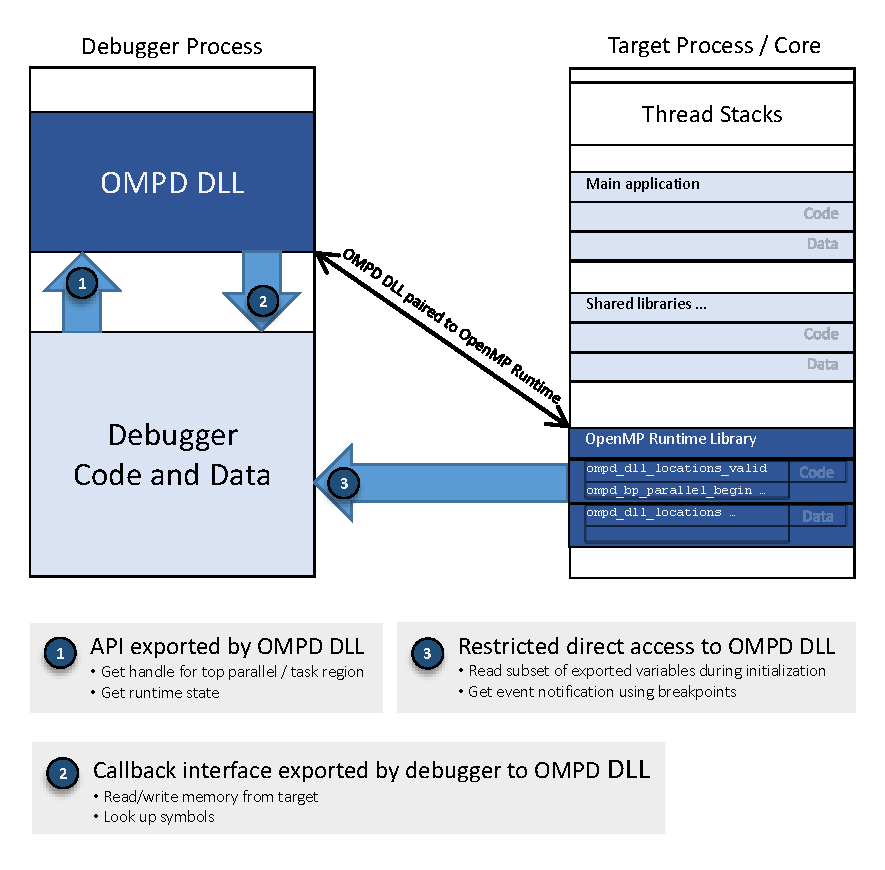
\includegraphics[width=6.0in,natwidth=424.8,natheight=417.6]{figures/ompd-structural-overview.pdf}
  \caption{OMPD: Structural overview}
\label{ompd-structural-overview:fig}
\end{figure}


\subsection{Design Scope}
\label{design-scope:sec}

The following OMPD API design is limited in scope to support
OpenMP~3.1 (or earlier) programs, and it cannot necessarily be applied
to OpenMP~4.0 (or later) programs due to the addition of \emph{target
regions} in OpenMP~4.0, which may include accelerator devices such as
GPUs.

However, the current OMPD API design allows for future
expansion of the OMPD API to support OpenMP~4.0, without breaking
compatibility or unnecessarily expanding its size or complexity.  To
this end, Section~\ref{ompd-concepts:sec} and
Figure~\ref{ompd-concepts:fig} include OMPD concepts that will be
required to support OpenMP~4.0 target regions in the future.
